\section{Теория}
	\subsection{Пошаговый метод}
	Система рассматривается в моменты времени, с $\Delta t$ разницей ---  $t_{i} = t_{i-1} + \Delta t$. В момент $t_i$ моделируются все события, которые должны были произойти с момента $t_{i-1}$, таким образом система приходит в состояние, соответствующее текущему времени. Преимуществом метода является простота его реализации. Очевидный минус - необходимость в анализе моментов времени без изменения в системе.
	
	\subsection{Событийный метод}
	Система также рассматривается дискретно, в моменты времени $t_i$, однако отличием от предыдущего метода является их выбор. Анализ системы производится только в моменты происхождения одного или нескольких событий. После выполнения соответствующих преобразований производится выбор $t_{i+1}$ как ближайшего из всех ожидаемых событий.

\section{Работа программы}
	Условием остановки поиска является обслуживание 1000 сообщений без изменения максимальной длины очереди.   
	
	В случае, если такое событие не происходит за 100 000 заявок, принимается, что генерация вместе с обратной связью помещают сообщения с большей интенсивностью, чем успевает обрабатывать их ОА. Следовательно, со временем длина очереди будет в среднем только расти, поэтому для любой выбранной очереди в определенный момент произойдут потери.
	
	Примеры работы программы приведены на рисунках \ref{pic:1}, \ref{pic:2} и \ref{pic:3}.
	
	\begin{figure}[h]
		\begin{center}
			{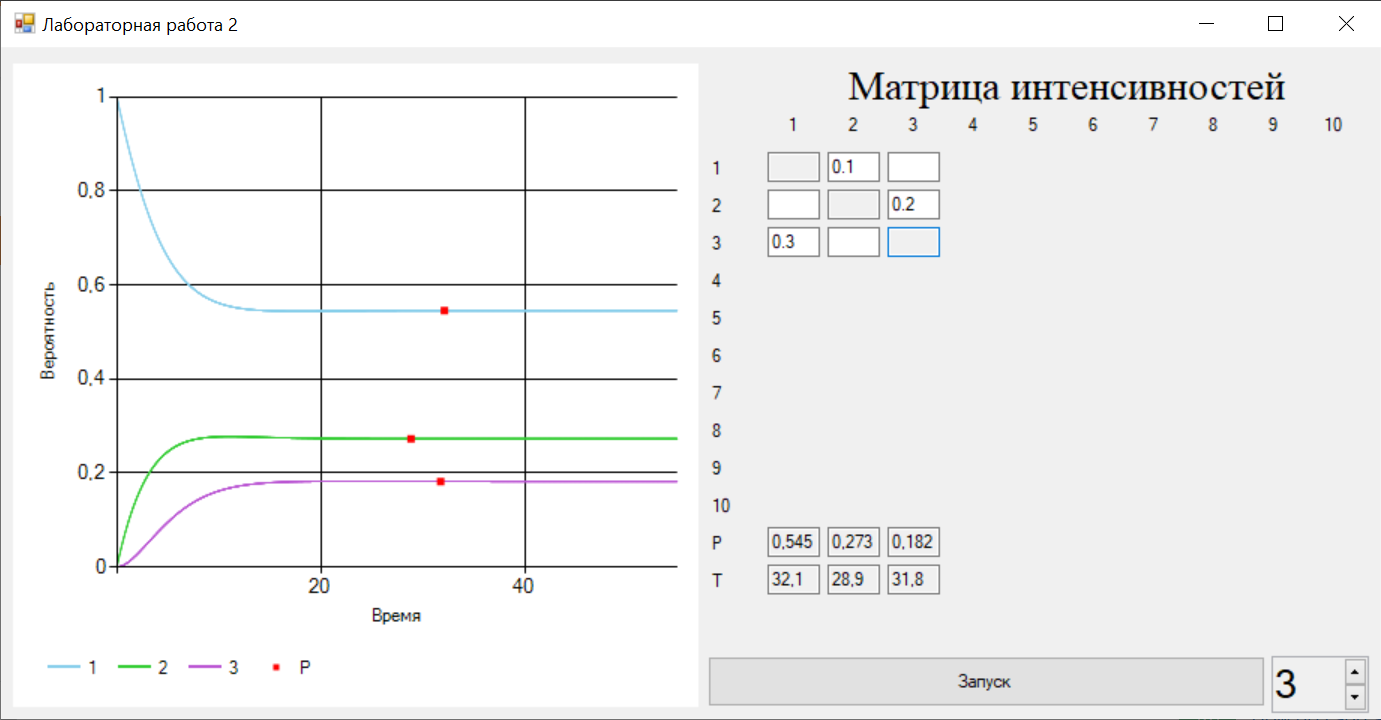
\includegraphics[scale=0.6]{1.png}
			\caption{Обслуживание в среднем быстрее генерации (Событийный метод)}
			\label{pic:1}}
		\end{center}
	\end{figure}

	\begin{figure}[h]
		\begin{center}
			{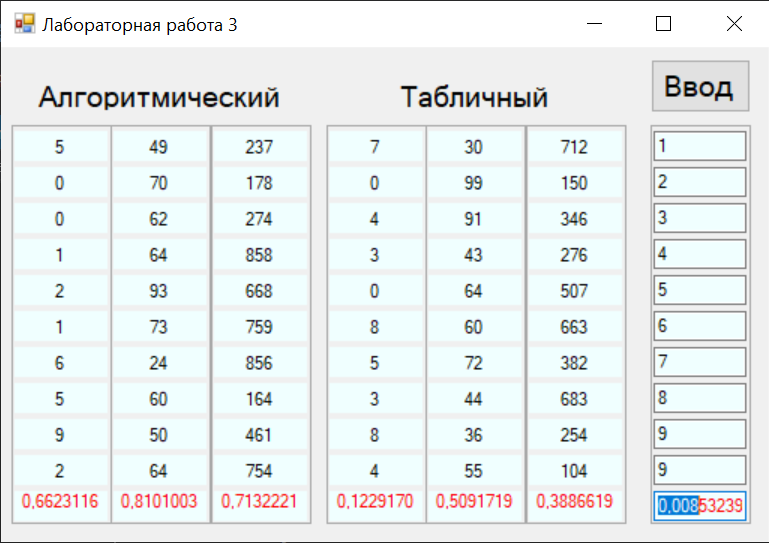
\includegraphics[scale=0.6]{2.png}
			\caption{Обслуживание в среднем быстрее генерации (Пошаговый метод)}
			\label{pic:2}}
		\end{center}
	\end{figure}

	В ходе экспериментов было установлено, что оба метода выдают одинаковый результат.
	
	\begin{figure}[h]
		\begin{center}
			{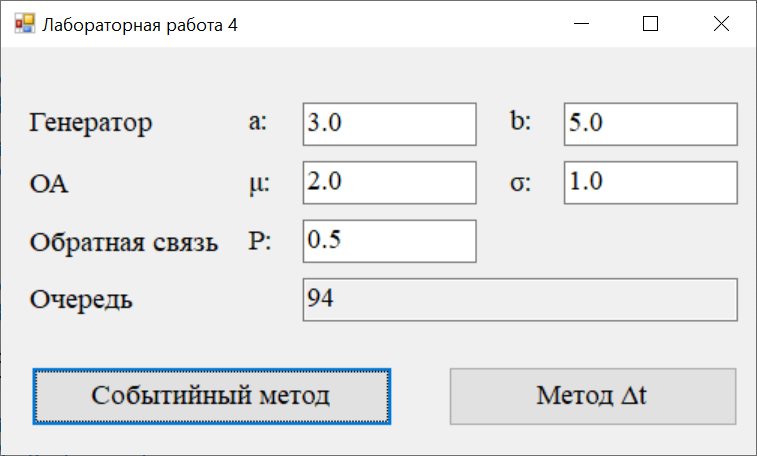
\includegraphics[scale=0.6]{3.png}
			\caption{Обратная связь 50\%}
			\label{pic:3}}
		\end{center}
	\end{figure}

	\begin{figure}[h]
		\begin{center}
			{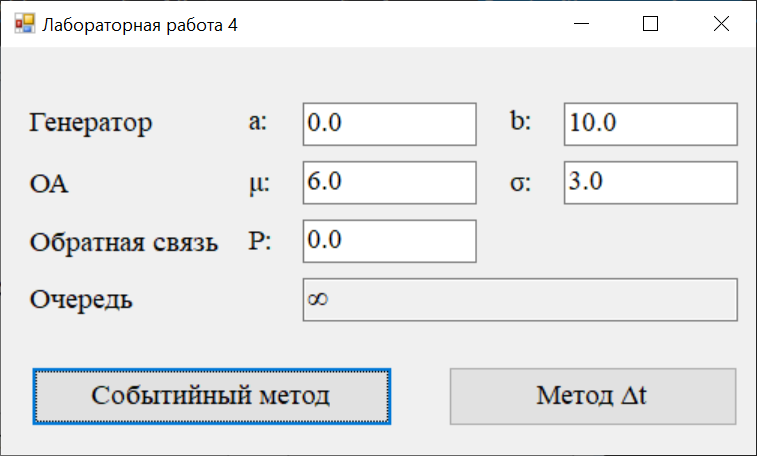
\includegraphics[scale=0.6]{4.png}
			\caption{Генерация интенсивнее обработки (размер очереди неопределён)}
			\label{pic:4}}
		\end{center}
	\end{figure}

	\begin{figure}[h]
		\begin{center}
			{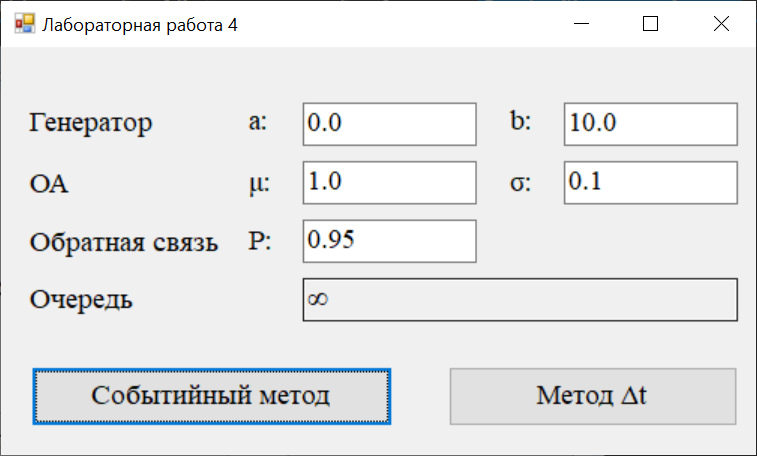
\includegraphics[scale=0.6]{5.png}
			\caption{Генерация и обратная связь интенсивнее обработки (размер очереди неопределён)}
			\label{pic:5}}
		\end{center}
	\end{figure}